% Created by tikzDevice version 0.12.3.1 on 2022-09-01 16:01:38
% !TEX encoding = UTF-8 Unicode
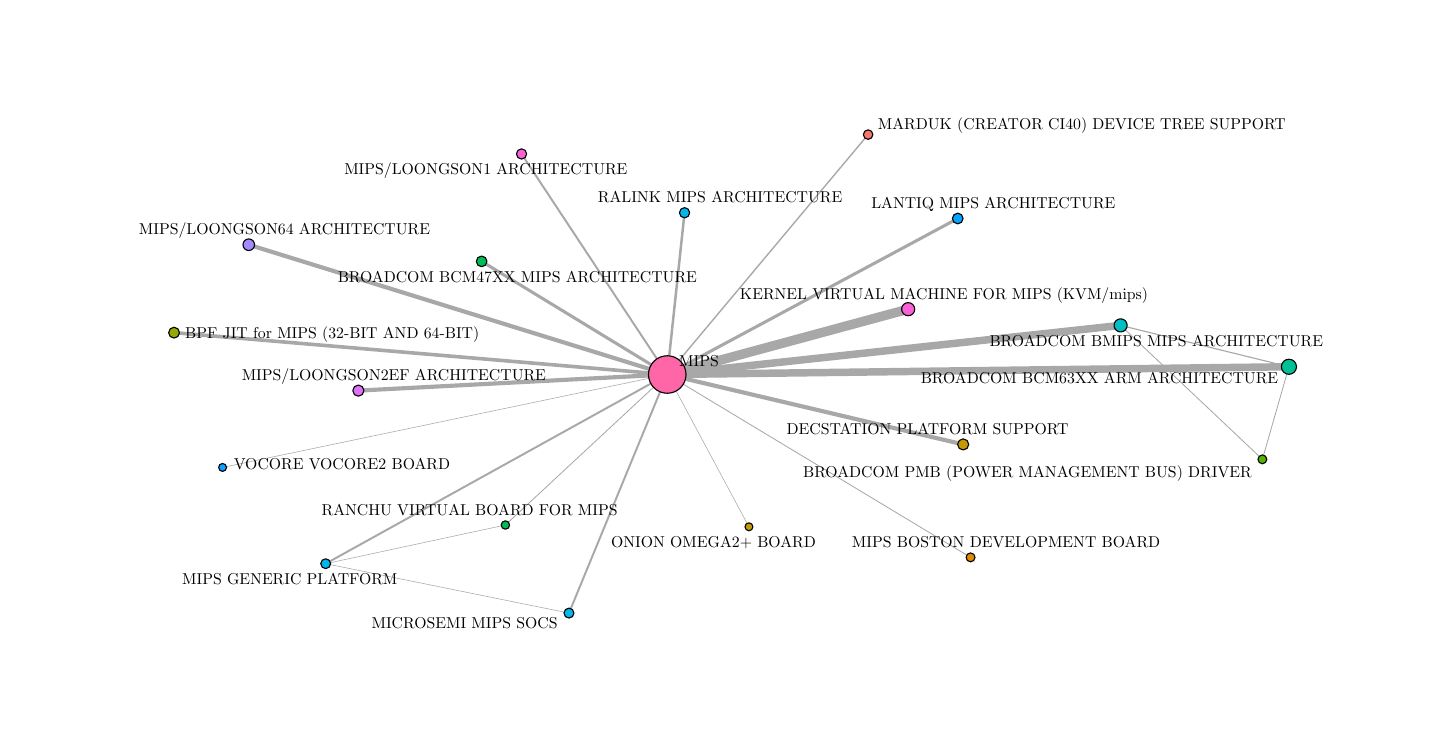
\begin{tikzpicture}[x=1pt,y=1pt]
\definecolor{fillColor}{RGB}{255,255,255}
\path[use as bounding box,fill=fillColor,fill opacity=0.00] (0,0) rectangle (505.89,252.94);
\begin{scope}
\path[clip] (  0.00,  0.00) rectangle (505.89,252.94);
\definecolor{fillColor}{RGB}{255,255,255}

\path[fill=fillColor] (  0.00,  0.00) rectangle (505.89,252.94);
\end{scope}
\begin{scope}
\path[clip] ( 32.75, 32.75) rectangle (475.89,222.94);
\definecolor{drawColor}{gray}{0.66}

\path[draw=drawColor,line width= 1.3pt,line join=round] ( 52.89,142.73) -- (231.11,127.61);

\path[draw=drawColor,line width= 1.1pt,line join=round] (164.04,168.49) -- (231.11,127.61);

\path[draw=drawColor,line width= 0.4pt,line join=round] (455.75,130.41) -- (394.93,145.36);

\path[draw=drawColor,line width= 0.3pt,line join=round] (455.75,130.41) -- (446.16, 96.95);

\path[draw=drawColor,line width= 2.7pt,line join=round] (455.75,130.41) -- (231.11,127.61);

\path[draw=drawColor,line width= 0.3pt,line join=round] (394.93,145.36) -- (446.16, 96.95);

\path[draw=drawColor,line width= 2.7pt,line join=round] (394.93,145.36) -- (231.11,127.61);

\path[draw=drawColor,line width= 1.5pt,line join=round] (338.04,102.35) -- (231.11,127.61);

\path[draw=drawColor,line width= 3.4pt,line join=round] (318.17,151.22) -- (231.11,127.61);

\path[draw=drawColor,line width= 1.1pt,line join=round] (336.08,183.98) -- (231.11,127.61);

\path[draw=drawColor,line width= 0.5pt,line join=round] (303.69,214.30) -- (231.11,127.61);

\path[draw=drawColor,line width= 0.7pt,line join=round] (195.59, 41.40) -- (231.11,127.61);

\path[draw=drawColor,line width= 0.2pt,line join=round] (195.59, 41.40) -- (107.68, 59.25);

\path[draw=drawColor,line width= 0.3pt,line join=round] (231.11,127.61) -- (340.71, 61.53);

\path[draw=drawColor,line width= 0.7pt,line join=round] (231.11,127.61) -- (107.68, 59.25);

\path[draw=drawColor,line width= 0.7pt,line join=round] (231.11,127.61) -- (178.46,207.31);

\path[draw=drawColor,line width= 1.5pt,line join=round] (231.11,127.61) -- (119.50,121.79);

\path[draw=drawColor,line width= 1.5pt,line join=round] (231.11,127.61) -- ( 79.89,174.51);

\path[draw=drawColor,line width= 0.2pt,line join=round] (231.11,127.61) -- (260.63, 72.58);

\path[draw=drawColor,line width= 0.9pt,line join=round] (231.11,127.61) -- (237.36,186.06);

\path[draw=drawColor,line width= 0.3pt,line join=round] (231.11,127.61) -- (172.62, 73.22);

\path[draw=drawColor,line width= 0.2pt,line join=round] (231.11,127.61) -- ( 70.43, 94.03);

\path[draw=drawColor,line width= 0.2pt,line join=round] (107.68, 59.25) -- (172.62, 73.22);
\definecolor{drawColor}{RGB}{0,0,0}
\definecolor{fillColor}{RGB}{153,168,0}

\path[draw=drawColor,line width= 0.4pt,line join=round,line cap=round,fill=fillColor] ( 52.89,142.73) circle (  1.96);
\definecolor{fillColor}{RGB}{0,188,86}

\path[draw=drawColor,line width= 0.4pt,line join=round,line cap=round,fill=fillColor] (164.04,168.49) circle (  1.93);
\definecolor{fillColor}{RGB}{0,192,148}

\path[draw=drawColor,line width= 0.4pt,line join=round,line cap=round,fill=fillColor] (455.75,130.41) circle (  2.73);
\definecolor{fillColor}{RGB}{0,191,196}

\path[draw=drawColor,line width= 0.4pt,line join=round,line cap=round,fill=fillColor] (394.93,145.36) circle (  2.37);
\definecolor{fillColor}{RGB}{83,180,0}

\path[draw=drawColor,line width= 0.4pt,line join=round,line cap=round,fill=fillColor] (446.16, 96.95) circle (  1.60);
\definecolor{fillColor}{RGB}{196,154,0}

\path[draw=drawColor,line width= 0.4pt,line join=round,line cap=round,fill=fillColor] (338.04,102.35) circle (  2.01);
\definecolor{fillColor}{RGB}{251,97,215}

\path[draw=drawColor,line width= 0.4pt,line join=round,line cap=round,fill=fillColor] (318.17,151.22) circle (  2.37);
\definecolor{fillColor}{RGB}{6,164,255}

\path[draw=drawColor,line width= 0.4pt,line join=round,line cap=round,fill=fillColor] (336.08,183.98) circle (  1.93);
\definecolor{fillColor}{RGB}{248,118,109}

\path[draw=drawColor,line width= 0.4pt,line join=round,line cap=round,fill=fillColor] (303.69,214.30) circle (  1.72);
\definecolor{fillColor}{RGB}{0,182,235}

\path[draw=drawColor,line width= 0.4pt,line join=round,line cap=round,fill=fillColor] (195.59, 41.40) circle (  1.80);
\definecolor{fillColor}{RGB}{255,102,168}

\path[draw=drawColor,line width= 0.4pt,line join=round,line cap=round,fill=fillColor] (231.11,127.61) circle (  6.78);
\definecolor{fillColor}{RGB}{227,137,0}

\path[draw=drawColor,line width= 0.4pt,line join=round,line cap=round,fill=fillColor] (340.71, 61.53) circle (  1.61);
\definecolor{fillColor}{RGB}{0,182,235}

\path[draw=drawColor,line width= 0.4pt,line join=round,line cap=round,fill=fillColor] (107.68, 59.25) circle (  1.78);
\definecolor{fillColor}{RGB}{251,97,215}

\path[draw=drawColor,line width= 0.4pt,line join=round,line cap=round,fill=fillColor] (178.46,207.31) circle (  1.85);
\definecolor{fillColor}{RGB}{223,112,248}

\path[draw=drawColor,line width= 0.4pt,line join=round,line cap=round,fill=fillColor] (119.50,121.79) circle (  2.02);
\definecolor{fillColor}{RGB}{165,138,255}

\path[draw=drawColor,line width= 0.4pt,line join=round,line cap=round,fill=fillColor] ( 79.89,174.51) circle (  2.09);
\definecolor{fillColor}{RGB}{196,154,0}

\path[draw=drawColor,line width= 0.4pt,line join=round,line cap=round,fill=fillColor] (260.63, 72.58) circle (  1.43);
\definecolor{fillColor}{RGB}{0,182,235}

\path[draw=drawColor,line width= 0.4pt,line join=round,line cap=round,fill=fillColor] (237.36,186.06) circle (  1.85);
\definecolor{fillColor}{RGB}{0,188,86}

\path[draw=drawColor,line width= 0.4pt,line join=round,line cap=round,fill=fillColor] (172.62, 73.22) circle (  1.52);
\definecolor{fillColor}{RGB}{6,164,255}

\path[draw=drawColor,line width= 0.4pt,line join=round,line cap=round,fill=fillColor] ( 70.43, 94.03) circle (  1.43);

\node[text=drawColor,anchor=base,inner sep=0pt, outer sep=0pt, scale=  0.57] at (110.05,140.78) {BPF JIT for MIPS (32-BIT AND 64-BIT)};

\node[text=drawColor,anchor=base,inner sep=0pt, outer sep=0pt, scale=  0.57] at (176.94,161.00) {BROADCOM BCM47XX MIPS ARCHITECTURE};

\node[text=drawColor,anchor=base,inner sep=0pt, outer sep=0pt, scale=  0.57] at (387.28,124.54) {BROADCOM BCM63XX ARM ARCHITECTURE};

\node[text=drawColor,anchor=base,inner sep=0pt, outer sep=0pt, scale=  0.57] at (407.83,137.91) {BROADCOM BMIPS MIPS ARCHITECTURE};

\node[text=drawColor,anchor=base,inner sep=0pt, outer sep=0pt, scale=  0.57] at (361.25, 90.39) {BROADCOM PMB (POWER MANAGEMENT BUS) DRIVER};

\node[text=drawColor,anchor=base,inner sep=0pt, outer sep=0pt, scale=  0.57] at (325.21,105.89) {DECSTATION PLATFORM SUPPORT};

\node[text=drawColor,anchor=base,inner sep=0pt, outer sep=0pt, scale=  0.57] at (331.12,154.76) {KERNEL VIRTUAL MACHINE FOR MIPS (KVM/mips)};

\node[text=drawColor,anchor=base,inner sep=0pt, outer sep=0pt, scale=  0.57] at (348.95,187.55) {LANTIQ MIPS ARCHITECTURE};

\node[text=drawColor,anchor=base,inner sep=0pt, outer sep=0pt, scale=  0.57] at (380.95,215.99) {MARDUK (CREATOR CI40) DEVICE TREE SUPPORT};

\node[text=drawColor,anchor=base,inner sep=0pt, outer sep=0pt, scale=  0.57] at (157.88, 35.77) {MICROSEMI MIPS SOCS};

\node[text=drawColor,anchor=base,inner sep=0pt, outer sep=0pt, scale=  0.57] at (242.56,130.58) {MIPS};

\node[text=drawColor,anchor=base,inner sep=0pt, outer sep=0pt, scale=  0.57] at (353.55, 65.11) {MIPS BOSTON DEVELOPMENT BOARD};

\node[text=drawColor,anchor=base,inner sep=0pt, outer sep=0pt, scale=  0.57] at ( 94.71, 51.74) {MIPS GENERIC PLATFORM};

\node[text=drawColor,anchor=base,inner sep=0pt, outer sep=0pt, scale=  0.57] at (165.56,199.81) {MIPS/LOONGSON1 ARCHITECTURE};

\node[text=drawColor,anchor=base,inner sep=0pt, outer sep=0pt, scale=  0.57] at (132.32,125.36) {MIPS/LOONGSON2EF ARCHITECTURE};

\node[text=drawColor,anchor=base,inner sep=0pt, outer sep=0pt, scale=  0.57] at ( 92.79,178.09) {MIPS/LOONGSON64 ARCHITECTURE};

\node[text=drawColor,anchor=base,inner sep=0pt, outer sep=0pt, scale=  0.57] at (247.80, 65.11) {ONION OMEGA2+ BOARD};

\node[text=drawColor,anchor=base,inner sep=0pt, outer sep=0pt, scale=  0.57] at (250.22,189.61) {RALINK MIPS ARCHITECTURE};

\node[text=drawColor,anchor=base,inner sep=0pt, outer sep=0pt, scale=  0.57] at (159.71, 76.80) {RANCHU VIRTUAL BOARD FOR MIPS};

\node[text=drawColor,anchor=base,inner sep=0pt, outer sep=0pt, scale=  0.57] at (113.57, 93.20) {VOCORE VOCORE2 BOARD};
\end{scope}
\end{tikzpicture}
